%In this section you will discuss the Technical Development related to your project.
%In one or more chapters you must describe fully the design and development strategies you have adopted and the results achieved.  You may refer to appropriate User and System documentation presented as appendices to avoid repeating extensive detail, so you can focus here instead on a discussion of your reasons for adopting the techniques and strategies you have followed.

%Again, it is difficult to give prescriptive guidance on the subsection structure you might adopt, as this will depend on the nature and content of your project.  However, you will probably want at least to consider sections addressing issues of System Design; Implementation; Testing.  If there is a lot to cover in any of these areas, it may warrant presentation as a full chapter rather than a section.

\chapter{Technical Development}

% Section Description:
%
\section{Tool Architecture}
Below is the system architecture for the degradation tool (See Section~\ref{ref:nfqueue} for NFQUEUE):

\begin{center}
	\newcommand{\width}{3cm}
\newcommand{\imageScale}{0.2}

\tikzset{%
  >={Latex[width=2mm,length=2mm]},
  % Specifications for style of nodes:
            base/.style = {rectangle, rounded corners, draw=black,
                           minimum width=\width, minimum height=1cm,
                           text centered, font=\sffamily},
            red/.style = {base, fill=red!15},
            blue/.style = {base, fill=blue!15}}
          

\begin{center}
\begin{tikzpicture}[node distance=1.5cm, every node/.style={fill=white, font=\sffamily}, align=center]

	\node(User)[xshift=-10cm]{\includegraphics[scale=\imageScale]{User}};		
	\node(UserText)[below of=User]{User};		
	
	\node(GUI)[base, right of=User, xshift=(\width), yshift=2cm]{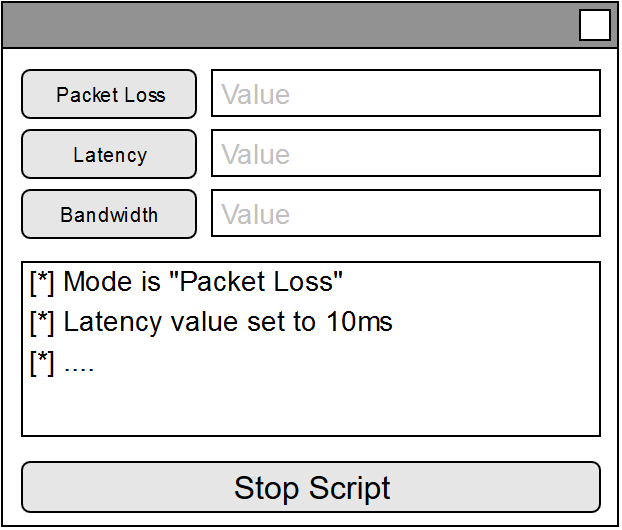
\includegraphics[scale=\imageScale]{Packet_UI_Design}};
	\node(GUIText)[below of=GUI, yshift=-0.5cm]{GUI};	
	
	\node(CLI)[base, below of=GUI, yshift=-2.25cm]{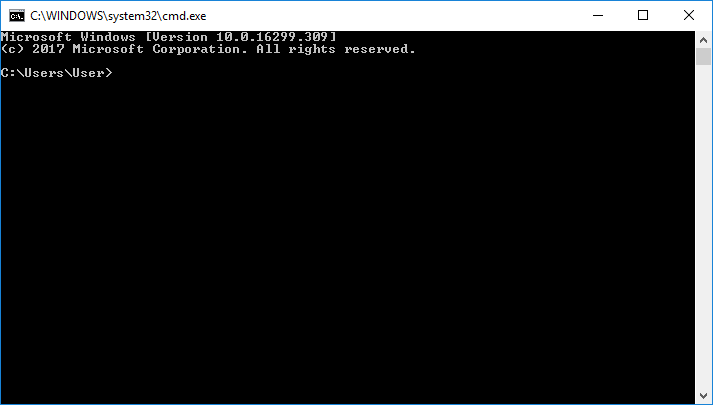
\includegraphics[scale=\imageScale]{CLI}};
	\node(CLIText)[below of=CLI]{CLI};
	
	\node(Effect)[blue, right of=User, xshift=(\width * 2) + 2cm]{Effect Choice};	
	\node(Nfqueue)[base, right of=Effect, xshift=(\width)]{NFQUEUE Creation};	
	
	\node(Parameters)[base, below of=Effect]{Parameter Handling};	
		
	
	\node(Packet)[red, below of=User, xshift=2cm, yshift=-4cm, text width=6cm]{Incomming Packets pushed into the NFQUEUE};
	\node(ChosenEffect)[blue, right of=Packet, xshift=\width + 2cm]{Chosen Effect};
	\node(PacketDescription)[above of=Packet, yshift=-0.5cm]{{\bf While NFQUEUE is running}};
	
	\draw[->] (User)--(GUI);
	\draw[->] (User)--(CLI);
	
	\draw[->] (GUI)--(Effect);
	\draw[->] (CLI)--(Parameters);
	\draw[->] (Parameters)--(Effect);	
	
	\draw[->] (Effect)--(Nfqueue);
	\draw[->] (Packet)--(ChosenEffect);
		
\end{tikzpicture}
\end{center}
	\begin{figure}[h]
		\caption{Architecture of the overall degradation tool}
	\end{figure}
\end{center}

It was decided early on that the script was to be controlled by two forms of interfaces; Graphical User Interface (GUI) and a text based Command Line Interface (CLI). This was to allow the tool to be run on the router (CLI) and also run on separate machines (GUI or CLI), making the tool versatile to many situations.

The system design is split into two stages:

\begin{itemize}
\item {\bf NFQUEUE Setup}\\
This section involves the creation of the NFQUEUE object, the binding of effect method to the queue and initialisation of variables dictating preferences.

\item {\bf NFQUEUE Running}\\
Each packet that is placed into the queue triggers this section, the handler is called that assigns a task to run the selected effect on the packet to one of the worker threads in a previously created thread pool. This allows custom effects simulation with filtering dynamically applied to all the packets.
\end{itemize}

\subsection{Parameter Handling}
Parameter handling is only required on the CLI due to the unrestricted input of the interface. Below is the activity diagram for the parameter handling process:

\begin{center}
	\newcommand{\widthParameter}{4cm}

\tikzset{%
	>={Latex[width=2mm,length=2mm]},
	% Specifications for style of nodes:
            base/.style = {draw=black,
                           minimum width=\widthParameter, 
                           text width=\widthParameter, 
                           minimum height=1cm, 
                           text centered},                           
            decision/.style = {base, diamond, fill=yellow!15},
            normal/.style = {base, rectangle, rounded corners}}

\begin{tikzpicture}

	\node (start) [shape=circle, fill=black]{};
	
	\node (command) [normal, right of=start, xshift=\widthParameter]{Command is entered};
	\node (parse) [normal, right of=command, xshift=\widthParameter]{Parameters are parsed};
	
	\node (correctParam) [decision, below of=parse, yshift=\widthParameter * -1]{Parameters Correct?};
	\node (showUsage) [normal, below of=correctParam, yshift=-\widthParameter, fill=red!15]{Show Usage and quit};
	\node (saveParam) [normal, left of=correctParam, xshift=-\widthParameter * 2]{Call coresponding argument method with arguments};

	\node (end) [shape=circle, fill=black, below of=saveParam, yshift=-\widthParameter]{};

	\draw[->] (start)--(command);
	\draw[->] (command)--(parse);
	\draw[->] (parse)--(correctParam);
	
	\draw[->] (correctParam)--node[fill=white]{No}(showUsage);
	\draw[->] (correctParam)--node[fill=white]{Yes}(saveParam);
	
	\draw[->] (saveParam)--(end);
	\draw[->] (showUsage)--(end);

\end{tikzpicture}
	\begin{figure}[h]
		\caption{UML Activity Diagram for parsing and handling parameters}
	\end{figure}	
\end{center}

The parameter handling as stated previously, is only required if the command line interface is used, this adds a little overhead in processing when using the command line but it is an unavoidable process. The error section when the `Usage' is printed will stop the entire program from continuing and will print a structured help message with the required format of the command. For most errors, human readable output will be produced to aid in debugging.

\subsection{Effect Choice \& NQUEUE Creation}

\begin{center}
	\newcommand{\widthEffectChoice}{4cm}

\tikzset{%
	>={Latex[width=2mm,length=2mm]},
	% Specifications for style of nodes:
            base/.style = {draw=black,
                           minimum width=\widthEffectChoice, 
                           text width=\widthEffectChoice, 
                           minimum height=1cm, 
                           text centered},                           
            decision/.style = {base, diamond, fill=yellow!15},
            normal/.style = {base, rectangle, rounded corners}}

\begin{tikzpicture}

	\node (start) [shape=circle, fill=black]{};
	
	\node (setQueue) [right of=start, normal, xshift=\widthEffectChoice]
	{Binds the NFQUEUE's `Mode' to chosen effect};
	
	\node (setVariables) [right of=setQueue, normal, xshift=\widthEffectChoice]
	{Sets all \\ preference \\ variables by parsed \\ arguments};
	
	\node (userOutput) [fill=blue!15, below of=setVariables, normal, yshift=-\widthEffectChoice + 2cm]
	{Displays summary of chosen modes and prefrences to the user};
	
	\node (runNfqueue) [left of=userOutput, normal, xshift=-\widthEffectChoice]
	{NFQUEUE Object is then run. That will pass all packets to the assigned 'Mode'};

	\node (end) [shape=circle, fill=black, below of=start, yshift=-\widthEffectChoice + 2cm]{};

	%Arrows
	\draw[->] (start)--(setQueue);
	\draw[->] (setQueue)--(setVariables);
	\draw[->] (setVariables)--(userOutput);
	\draw[->] (userOutput)--(runNfqueue);
	\draw[->] (runNfqueue)--(end);

\end{tikzpicture}
	\begin{figure}[h]
		\caption{UML Activity Diagram for assigning the choice of effect}
	\end{figure}
\end{center}


Choosing a mode for the program gives the ability to switch between degradation effect and arrangement of effects. This process is exactly the same for GUI and CLI. This is due to the shared code between the different user interfaces, all the CLI does is parse arguments and calls the correct methods and the GUI just directly calls these methods when buttons are clicked.

\subsection{Incoming Packets}
\begin{center}
	\begin{tikzpicture}

	\node (start) [shape=circle, fill=black]{};
	
	\node (handler) [normal, right of=start, xshift=\width * 2] 
	{Packet placed into queue caught by handler method};
	
	\node (filterSet) [below of=handler, yshift=-\width, decision] {Is packet filter set?};
	\node (targetCheck) [left of=filterSet, xshift=-\width * 2, normal]{Check filter against packet};
	\node (passFilter) [below of=targetCheck, yshift=-\width, decision]{Does packet pass filter};
	
	\node (runEffect) [below of=filterSet, yshift=-\width, normal, fill=red!15]
	{Run assigned \\ effect on packet};	
	
	\node (Accept) 	[fill=blue!15, below of=passFilter, normal, yshift=-\width]{Accept Packet};
	\node (Drop)	[fill=blue!15, below of=runEffect, normal, yshift=-\width]{Drop Packet};	
	
	%Find the middle between the two nodes
 	\coordinate (CENTER) at ($(Accept)!0.5!(Drop)$);		
	\node (end)	[below of=CENTER, shape=circle, fill=black, yshift=-2cm]{};	
	
	\node (endLabel) [below of=end]{Thread released};	
	
	% Connections
	\draw[->] (start)--(handler);
	\draw[->] (handler)--(filterSet);
	
	\draw[->] (filterSet)--node[fill=white]{Yes}(targetCheck);
	\draw[->] (filterSet)--node[fill=white]{No}(runEffect);
	
	\draw[->] (targetCheck)--(passFilter);
	
	\draw[->] (passFilter)--node[fill=white]{Yes}(runEffect);
	\draw[->] (passFilter)--node[fill=white]{No}(Accept);	

	\draw[->] (runEffect)--(Accept);
	\draw[->] (runEffect)--(Drop);
	
	\draw[->] (Drop)--(end);
	\draw[->] (Accept)--(end);	
s
\end{tikzpicture}
	\begin{figure}[h]
		\caption{Activity diagram for running an effect on a single packet}
		\label{ref:incommingAD}
	\end{figure}
\end{center}

Figure~\ref{ref:incommingAD} shows the activity diagram for the process of running an effect on a single packet. The script automatically effects every packet that is placed in the NFQUEUE, this means protocol support does not need to be managed and no code manipulating or monitoring sockets is required.

% Section Description:
%
\section{Tool Class Design}
\subsection{Effect Class Diagram}

\begin{center}
	\begin{tikzpicture}

% Effect - Parent class
\umlclass{Effect}
{
	+ allow\_print 		: bool \\ 
	+ accept\_packets 	: bool
}
{
	+ print()			: void \\
	+ print\_stats()	: void \\
	+ effect()			: void 	
}

\umlclass[below right= 2cm of Effect]{Latency}
{
	+ latency\_value\_ms : int
}

\umlclass[below = 1.45cm of Effect]{PacketLoss}
{
	+ packet\_loss : int
}

\umlclass[below left= 2cm of Effect]{Bandwidth}
{
	+ rate\_limit : int
}

% Links
\umlVHVinherit{Effect}{Latency}
\umlVHVinherit{Effect}{PacketLoss}
\umlVHVinherit{Effect}{Bandwidth}

\end{tikzpicture}
	\begin{figure}[h]
		\caption{UML Class diagram for producing degradation effects}
	\end{figure}
\end{center}

The above design is for the various effects that will be implemented into the program. They will be self contained within separate modules encased in an object. This was chosen so each effect is modular and self contained from one another. The modularity will improve the potential readability and maintainability of the code base, it will also make the code base much more scalable where effects can be added with high speed because of the lack of repeated code.  Each effect will inherit from the base class ``Effect", where it will obtain methods and properties used for functionality and boolean variables for allowing printing and accepting packets. These boolean variables are necessary when `chaining' effects together, where a packet can only be accepted once and only a single print will be required.

\clearpage
\subsection{Tool Activity Diagram}
\begin{center}
	\begin{tikzpicture}
	\node (start)[shape=circle, fill=black]{};	
	\node (scriptStarted)[normal, right of=start, xshift=\width]{Script is started};
	\node (parameters)[normal, right of=scriptStarted, xshift=\width]
	{Parameters are parsed and processed};	
	\node (validParam)[decision, right of=parameters, xshift=\width + 2cm]{Valid \\ parameters?};
	\node (startRunning)[normal, below of=validParam, xshift=-\width, yshift=-\width]
	{Start running effect with selected params};
	\node (quit)[normal, below of=validParam, yshift=(-\width * 3) - 0.5cm]
	{Quit and show usage()};
	\node (sigintSent)[decision, left of=startRunning, xshift=-\width * 2]{SIGINT sent?};
	\node (showCleanQuit) [normal, below of=sigintSent, yshift=-\width]
	{Show clean quit message};
	\node (end) [circle, below of=showCleanQuit, fill=black, yshift=-\width / 2]{};

	%Lines
	\draw[->] (start)--(scriptStarted);
	\draw[->] (scriptStarted)--(parameters);
	\draw[->] (parameters)--(validParam);
	\draw[->] (startRunning)--(sigintSent);

	\draw[red, ->] (validParam)\yesLink{startRunning};
	\draw[red, ->] (validParam)\noLink{quit};	
	\draw[red, ->] (sigintSent) edge [loop left] node[swap] {No}();
	
	\draw[red, ->] (sigintSent)\yesLink{showCleanQuit};
	\draw[->] (showCleanQuit)--(end);
	\draw[->] (quit)--(end);


\end{tikzpicture}
	\begin{figure}[h]
		\caption{Activity Diagram for the degradation tool}
		\label{ref:ToolAD}
	\end{figure}
\end{center}

Figure~\ref{ref:ToolAD} above is the activity diagram for the tool that will implement the effect classes above. This tool will be utilised directly from the command line or run by the GUI. The decision of having a single script that is controlled by multiple approaches allows for one central point of functionality and means code can be shared throughout the project. Figure~\ref{ref:ToolAD} shows the design choices for the direct control on the script. SIGINT is mentioned in the centre of the diagram, SIGINT is a built in signal in the Linux operating system that represents an interrupt signal, where it is triggered by pressing ``Control + C", this is the most common/clean way of stopping a script. The other alternatives to closing the script ``Control + Z" (SIGTSTP) and ``Control + /" (SIGQUIT) will be remapped to send a SIGINT signal and perform the same role, this will mean the program has one tidy point of closure.

% Section Description:
%
\section{Tool UI Design}
\begin{wrapfigure}{R}{5cm}
\begin{center}
	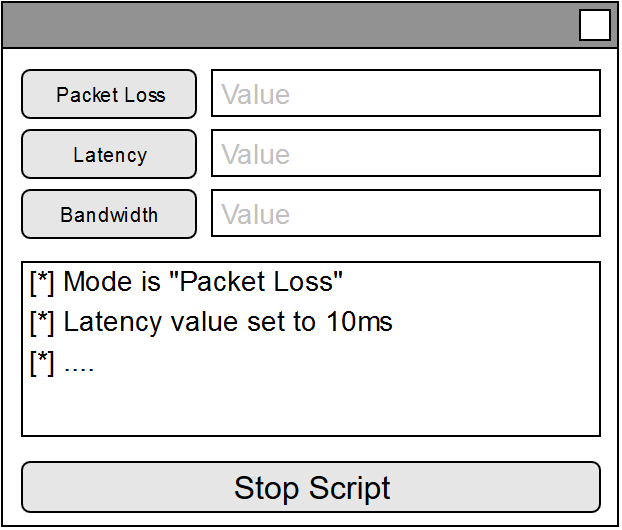
\includegraphics[scale=0.3]{Packet_UI_Design}
	\caption{Initial user interface design for the Degradation GUI}
	\label{ref:planUI}
	\paragraph{}
	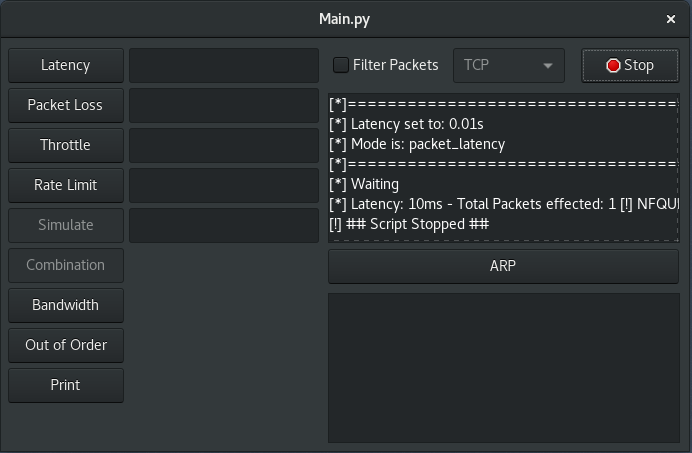
\includegraphics[scale=0.3]{live_packet_ui}
	\caption{Actual working Packet user interface}
	\label{ref:workingUI}
\end{center}	
\end{wrapfigure}

The UI is one of the ways to control the degradation. The UI needs to have a way to easily include new controls that link up to parameters in the script, thus making the interface scalable and easy to maintain. A text box is required to display the same output as the terminal window, this can be achieved by `piping' the stdout to a custom section of the user interface. The `stdout' is the data stream that links up to a Linux terminal window, if the stdout points to somewhere else it will display where it is needed. Figure~\ref{ref:planUI} shows the initial drafted design for the user interface.

Figure~\ref{ref:workingUI} contains the actual working user interface for the script. The design has been followed to some extent with only changes occurring in the layout of the controls on the left side designed to make it much easier to include new effects in the future. The inclusion of a window and output text box designed to allow ARP spoofing to occur has also been included in the working user interface.

% Section Description:
%
\section{Tool Implementation}
The tool performs the degradation effect on the computer it is running on, the script is written in Python 3.6 \citep{pranskevichuspython} and can be run on a computer running a Linux based OS with the required version of the Python interpreter installed.


\subsection{NFQUEUE}
\label{ref:nfqueue}
The script utilises a section in the Linux kernel referred to as the ``NFQUEUE". This is as the name suggests a queue that is stored in kernel memory that will store up packets until the user provides one of the two verdicts: `Drop' or `Accept'. The packets are pushed into this queue by the use of `iptable' rules. Iptabales is a tool designed to filter packets by criteria. Figure~\ref{ref:iptables} contains a flow diagram for the path a packet might take through a system, each table can have filtering rules embedded into to it:

% Diagram
%Variables
\newcommand{\nodefont}{\rmfamily}
\newcommand{\normalWidth}{3cm}

%----------------------------------------%
%  IPtables Diagram						 %
%----------------------------------------%
\tikzset{%
  >={Latex[width=2mm,length=2mm]},
  % Specifications for style of nodes:
            base/.style = {rectangle, rounded corners, draw=black,
                           minimum width=4cm, minimum height=1cm,
                           text centered, font=\sffamily}, 
            process/.style = {base, minimum width=\normalWidth, fill=orange!15,
                           font=\nodefont},
            network/.style = {base, fill=blue!15},
            local/.style = {base, fill=red!15}}
\vspace{0.25cm}                
\begin{center}
\begin{tikzpicture}[node distance=1.5cm, every node/.style={fill=white, font=\sffamily}, align=center]
    	\node(NetworkCard)[network]{Network Card};
        \node(NetworkCardOut)[network, right of=NetworkCard, xshift=6cm]{Network Card};
        
    	\node(PreRouting)[process, below of=NetworkCard]{Pre-Routing};
    	\node(Forward)[process, right of=PreRouting, xshift=2.5cm, yshift=-1.75cm]{Forward};
    	\node(Input)[process, below of=PreRouting, yshift=-2cm]{Input};
        \node(PostRouting)[process, right of=PreRouting, xshift=6cm]{Post-Routing};
    	\node(Output)[process, right of=Input, xshift=6cm]{Output};
        
        \node(LocalProcessIn)[local, below of=Input]{Local Process};
        \node(LocalProcessOut)[local, below of=Output]{Local Process};
        
        %In Arrows
        \draw[->] (NetworkCard)--(PreRouting);
        \draw[->] (PreRouting)|-(Forward);
        \draw[->] (PreRouting)--(Input);
        \draw[->] (Input)--(LocalProcessIn);
        
        %Out Arrows
        \draw[->] (LocalProcessOut)--(Output);
        \draw[->] (Output)--(PostRouting);
        \draw[->] (Forward)-|(PostRouting);
        \draw[->] (PostRouting)--(NetworkCardOut);        
\end{tikzpicture}
\end{center}   
\begin{figure}[h]
	\caption{Diagram showing the iptables map}
	\label{ref:iptables}
\end{figure}

If there was a case where all packets entering the machine need filtering, an iptable rule would be added to the "Pre-Routing" section of the table to catch all packets entering the machine. 

To move all packets entering from the network card into the NFQUEUE the iptable rule would be added like so:
\begin{center}
	\begin{console_font}
		\large{iptables -A INPUT -j NFQUEUE}
	\end{console_font} 
\end{center}
Where `-A tells iptables to append a rule onto the `INPUT' table and `-j' is the rule that affects the packet, in this case pushing it into the default queue.

This forms the main component of the functionality of the script. A series of iptable rules that filter packets into the NFQUEUE and allow to script to perform verdicts on each packet separately. This per packet verdict allows for effects to be easily applied to packets entering and leaving the machine.

Below is code for the creation of the NFQUEUE object along side the iptable rules:
\begin{Code}[]{NFQUEUE}
# iptables
os.system("iptables -A INPUT -j NFQUEUE")
os.system("iptables -t nat -A POSTROUTING -j NFQUEUE")

# Setup for the NQUEUE
nfqueue = NetfilterQueue()

try:
	nfqueue.bind(0, mode)  # 0 is the default NFQUEUE
except OSError:
	print_force("[!] Queue already created")
	
nfqueue.run()
\end{Code}
\begin{figure}[h]
	\caption{Programmatically creating an NFQUEUE}
\end{figure}

In the code above, the variable {\code mode} contains a method that performs effects on the packets. Figure~\ref{ref:latencyMode} shows what {\code mode} would equal if the effect chosen was latency.

The two iptable rules were chosen due to their coverage; they cover all incoming packets to the router (INPUT) and all packets being routed and coming directly from the router (POST-ROUTING). These rule also don't cause the same packet to be pushed into the queue more than once.

\begin{Code}{Latency Packet Mode}
def packet_latency(packet):
    """This function is used to incur latency on packets"""
    if affect_packet(packet):
        assign_thread(latency_obj.effect, [[packet, time.time()]])
    else:
        packet.accept()
\end{Code}
\begin{figure}[h]
	\caption{Example of a potential structure of a {\code Mode}}
	\label{ref:latencyMode}
\end{figure}

There are a couple of aspects to note in the above code listing:
{\code affect\_packet} is the method that checks the packet against the active filters. 
{\code assign\_thread} is the method that assigns the object effect method ({\code latency\_obj.effect}) to an idle thread in the pool and {\code packet.accept()} and {\code packet.drop()} are the ways the packet is assigned a verdict. This verdict can be assigned at any point in the code and becomes instantly active.

\clearpage
\subsection{Degradation Effects}
The script contains the functionality to simulate a plethora of effects. Each effects functionality will be described below. It is of note that any of these effects can be chained together in any order.

\subsubsection{Latency}
Latency as described in the background section, is the delay in initiating a task and seeing its results. Latency is simulated by using a timing mechanism where the arrival time of the packet is saved. The packet is then pushed into the NFQUEUE that triggers a single thread that will hold the packet for a set amount of time. The holding time is calculated by subtracting the amount of time the packet has already been in the script away from the target time. The packet is then marked as `ACCEPTED' and pushed out of the queue.

\begin{Code}{Latency}
def custom_effect(self, packet):
	"""Thread functionality"""

	# # Dynamic time mode
	# Parameters contained within a single object
	if type(packet) is list:
		packetObj = packet[0]
		startTime = packet[1]

		# Works out the time difference between
		# thread conception and now
		elapsed = time.time() - startTime
            
		# Take the elapsed time off the target
		wait_time = self.latency_value - elapsed

		if wait_time < 0:
			# No waiting			
			pass
		else:
			time.sleep(wait_time)
			
		self.accept(packetObj)
			
	# # Static time mode
	else:
		time.sleep(self.latency_value)
		self.accept(packet)

\end{Code}
\begin{figure}[h]
	\caption{Code that simulates latency on a connection}
\end{figure}

\subsubsection{Packet Loss}
Packet loss is simulated by first assigning a target value, lets say for this example, 10\%. For each packet the script randomly generates a number between 1 and 100, if that value is less than the target value the packet is dropped, and if the value is larger the packet is accepted. This therefore, creates the effect of packet loss. It does, however, require a fair amount of packets to balance out statistically and reach the percentage target.

\begin{Code}{Packet Loss}
def custom_effect(self, packet):
        """This function will issue packet loss,
           a percentage is defined where lower 
           values are dropped and higher values are accepted"""

        if self.packet_loss_percentage != 0:

            # random value from 0 to 100
            random_value = random.uniform(0, 100)

            if self.packet_loss_percentage > random_value:
                self.dropped_packets += 1
                packet.drop()

            else:
                self.accept(packet)
        else:
            self.accept(packet)
\end{Code}
\begin{figure}[h]
	\caption{Code that causes packet loss on all incoming traffic}
\end{figure}

\subsubsection{Bandwidth}
There are two modes created for bandwidth; rate limiting and a simple display. Rate limiting allows the script to limit the rate of bandwidth flowing through the machine and calculates the rate transferred over a period of 5 seconds, if the rate is higher it waits until the rate drops below the target. This gives it the ability to adjust quickly and allows the script to be run for a long period of time without the overall average of the bandwidth affecting future changes. Displaying the bandwidth works exactly the same but without the limit check, this is useful when checking the current download speeds or the max transfer rate.

Limiting bandwidth is displayed in Figure~\ref{ref:BandwidthCode} below:

\begin{Code}{Bandwidth Limit}
def custom_effect(self, packet):
	"""Used to limit the bandwidth"""

	# Adds packet to the backlog
	self.packet_backlog.append(packet)
	
	# The algorithm will send until the backlog is empty or 
	# the limit is exceeded
	while self.rate < self.bandwidth and len(self.packet_backlog) > 0:
		self.send_packet(self.packet_backlog[0])
            
		# Packet is removed from the list
		del self.packet_backlog[0]
			
		self.calculate_rate_overall_avg()
\end{Code}
\begin{figure}[h]
	\caption{Code that is used to limit the bandwidth of a connection}
	\label{ref:BandwidthCode}
\end{figure}

\subsubsection{Out-of-order}
This effect changes the order of packets coming into the script, this can be used to check its effect on UDP and TCP and can test how quickly these issue can be rectified. It works by queuing up every packet into a list, then a single thread randomly picks an index of that list, accepts the packet and allows it to leave. This, therefore, means at its most extreme the order can be last in, first out.

\subsubsection{Connection Simulation}
Connection simulation isn't quite a degradation effect but its intent is to simulate the effect of degradation on a common connection like `WiFi` or a 3G connection to see how these are affected by the aforementioned degradation effects. This can be useful in some situations where, for example, testing a mobile applications performance over 3G with heavy latency, the mobile would connect to the script and the script would effect any traffic entering or leaving the handset.

The types of connections were simulated using common values for latency and packet loss. 3G, 4G and WiFi values were obtained from Ofcom studies \citep{ofcom} \citep{ofcomMobile}.

\subsubsection{Jitter}
Jitter mode clumps and separates packets in their transmission. Therefore, causing variation in inter packet timing. This is required test how the protocol deals with jitter in the connection. Jitter as explained in the background is the intra-packet latency i.e. the difference in time between arrivals of packets.

\subsection{ARP Spoofing}
\label{ref:arpSpoof}
The script also supports an ARP spoofing mode that allows it to sit between a gateway and a specified target. This means the script can perform all its functions on a single target with a very quick deployment time. As touched on in the background (See Section ~\ref{ref:arp_background}) the ARP protocol performs no authentication on any changes to the ARP cache meaning that you can perform a man in the middle attack and route traffic through a machine of your choice.

The script begins by grabbing the MAC addresses connected to the provided gateway and target IP addresses. Two ARP reply packets (denoted by the `2' opcode) are sent out. One packet telling the victim that the current machines MAC address maps to the gateway, and the other packet telling the gateway that the victims IP maps to the current machines MAC address.

Below is the process visualised:




% Gateway
\newcommand{\GatewayLabel}{
\begin{tabular}{l l}
Gateway\\
\hline
\vspace{0.1cm}
\bf{192.168.1.1} & \bf{C8:49:BD:82:47:4D}\\
ARP Cache\\
\hline
192.168.1.2 & 46:41:73:EC:70:E3
\end{tabular}
}

%Victim
\newcommand{\VictimLabel}{
\begin{tabular}{l l}
Victim\\
\hline
\vspace{0.1cm}
\bf{192.168.1.2} & \bf{46:41:73:EC:70:E3}\\
ARP Cache\\
\hline
192.168.1.1 & C8:49:BD:82:47:4D
\end{tabular}
}

\begin{center}
\begin{tikzpicture}[
    diagram item/.style={},
    align=left
]         

\node (Router)[
    diagram item,
    label=above:\GatewayLabel,
    yshift=-2cm
] {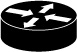
\includegraphics[scale=\ciscoImageScale]{\cisco/router}};

\node (Victim)[
	diagram item,
	label=above:\VictimLabel,
	right of=Router,
	xshift=7cm
] {
\includegraphics[scale=\ciscoImageScale]{\cisco/workstation}};


\draw[-] (Router)--(Victim);

\end{tikzpicture} 
\end{center}


\begin{figure}[h]
	\caption{Diagram displaying ARP Cache of a small network}
	\label{ref:arp_before}
\end{figure}

Figure~\ref{ref:arp_before} shows both connected ends have gone through the process to resolve the IP addresses to MAC addresses, you can see above each device their corresponding IP, MAC and ARP Cache. The ARP cache, as mentioned previously, is a record linking IP addresses to MAC addresses.

\newcommand{\tgap}{0.1cm}

% Gateway
\newcommand{\GatewayLabelAfter}{
\begin{tabular}{l l}
Gateway\\
\hline
\vspace{\tgap}
\bf{192.168.1.1} & \bf{C8:49:BD:82:47:4D}\\
ARP Cache\\
\hline
192.168.1.2 & \bf{\textcolor{red}{37:A8:22:F6:BB:34}} \\
192.168.1.3 & 37:A8:22:F6:BB:34
\end{tabular}
}

%Victim
\newcommand{\VictimLabelAfter}{
\begin{tabular}{l l}
Victim\\
\hline
\vspace{\tgap}
\bf{192.168.1.2} & \bf{46:41:73:EC:70:E3}\\
ARP Cache\\
\hline
192.168.1.1 & \bf{\textcolor{red}{37:A8:22:F6:BB:34}} \\
192.168.1.3 & 37:A8:22:F6:BB:34
\end{tabular}
}

%Attacker
\newcommand{\AttackerLabel}{
\begin{tabular}{l l}
Attacker\\
\hline
\bf{192.168.1.3} & \bf{37:A8:22:F6:BB:34} 
\end{tabular}
}

\begin{center}
\begin{tikzpicture}[
    diagram item/.style={},
    align=left
]         

\node (Router)[
    diagram item,
    label=above:\GatewayLabelAfter,
    yshift=-2cm
] {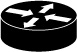
\includegraphics[scale=\ciscoImageScale]{\cisco/router}};

\node (Victim)[
	diagram item,
	label=above:\VictimLabelAfter,
	right of=Router,
	xshift=7cm
] {
\includegraphics[scale=\ciscoImageScale]{\cisco/workstation}};


%Find the middle between the two nodes
\coordinate (CENTER) at ($(Victim)!0.5!(Router)$);		
\node (Attacker)[
	label=below:\AttackerLabel,
	below of=CENTER,
	yshift=-3.5cm
] {
\includegraphics[scale=\ciscoImageScale]{\cisco/laptop}};

\draw[red, very thick] (Router)--(Attacker);
\draw[red, very thick] (Attacker)--(Victim);


\end{tikzpicture} 
\end{center}


\begin{figure}[h]
	\caption{Diagram visualising the ARP Tables after a spoofing attack}
	\label{ref:arp_after}
\end{figure}

After the 3rd device connects to the network, both devices gain a record of its IP and MAC address in their ARP cache. 

After both spoofed packets have been sent out, the ARP cache for each receiving end gets updated. The text in red of Figure~\ref{ref:arp_after} shows the changes caused by the spoofed ARP packets. Now when either end wants to talk to each other it will resolve the MAC address and send it with the new MAC address in the table, this will therefore, get routed through the attacking PC and will allow the script to receive all the traffic between the two parties.

\subsection{Network Attacks}
Two network attacks were implemented into the script, these served the purpose of providing very heavy artificial traffic designed to create heavy loads or interfere with integral protocols. Not many attacks were added as they do not provide much purpose apart from stress testing and they reside on the edge of the scope of this project. There will also be a brief discussion into possible techniques to mitigate the effects. 

\subsubsection{UDP Flooding}
UDP flooding is a very simple attack, lots of UDP packets are created and sent over a network stream very quickly. This attack is designed to `flood' the buffers in the receiving machine and slow down an internet connection. The script creates 10 or so threads that create and send packets concurrently, this amount of threads easily reaches the max throughput of the test machines NIC card and massively reduces internet connection on the receiving end.

The attack could be detected and prevented by a script that monitors the network transfers rates, this attack will create a huge spike in the transfer rate that can be detected and all traffic would be blocked from the sending party.

\begin{Code}{UDP Flooding}
  def effect(self):
        """The main body of the attack"""

        # Destination
        port = random.randint(0, 65535)

        # Creates a UDP packet with 1024 bytes of random data
        # Scapy is used to construct the packet
        pkt = bytes(IP(dst=self.target_ip) / UDP(sport=52, dport=port) / 
        			Raw(load=random._urandom(1024)))

        sock = socket.socket(socket.AF_INET, socket.SOCK_DGRAM)

        while self.running:

            # Uses the previously created socket to send
            sock.sendto(pkt, (self.target_ip, port))
			
\end{Code}
\begin{figure}[h]
	\caption{Code displaying the sending of UDP packets}
	\label{ref:UdpFloodingFigure}
\end{figure}

Figure~\ref{ref:UdpFloodingFigure} above is a section of code from the UDP flooding attack script. As mentioned previously around 10 threads will run the code at the same time in an attempt to maximise the throughput of UDP packets. The effects of the attack are visible on the target end and causes a visual degradation in the connection speed.

\subsubsection{ARP Spamming}
This attack works by once again exploiting the lack of authentication of the ARP protocol. In the entire network mode the script starts by detecting all active hosts on a network, it then starts sending out falsified ARP reply packets with randomly generated MAC addresses inside. This results in all computers on the networking having incorrect ARP cache values and resulting in computers incorrectly resolving IP and MAC address combinations and traffic being blocked.

\begin{Code}{ARP Spamming}
def start(self):
   while self.running:
        
       # Talks to every machine and changes the ARP value
       # The list of hosts is obtained by an NMAP scan
       for host_dst in self.active_hosts:
           for host_src in self.active_hosts:
           	  if host_dst != host_src:
                 
           	  	# Send the ARP packet - rnd_mac_addresses() creates
           	  	# a fully random  MAC address
           	  	self.send_arp_packet(host_dst, 
                                    host_src, 
                                    self.rnd_mac_addresses[count])


def send_arp_packet(self, dst, src, mac, op_code=2):
        
    # Construction of the ARP Packet
    pkt = ARP(op=2, 
              pdst=dst, 
              psrc=src, 
              hwdst="ff:ff:ff:ff:ff:ff", 
              hwsrc=mac)

    send(pkt, verbose=0)
					
\end{Code}
\begin{figure}[h]
	\caption{Code from the ArpSpamming.py script}
	\label{fig:ArpSpammingCode}
\end{figure}


Figure~\ref{fig:ArpSpammingCode} above shows the attack effecting the entire network. The scan finds all active hosts and returns them as a list that is then used as source and destination IP addresses that ultimately end up affecting the entire local networks ARP cache.

This attack is relatively easy to execute but can simply be prevented by issuing static ARP tables for each machine, with a few authenticated machines allowed to perform changes. This static table prevents unsolicited ARP replies from changing IP and MAC address combinations and also prevents ARP Spoofing from occurring on that network.


\subsection{Router Design}
The router is required to create an access point and allow access to the internet. Traffic will be routed through the router that is destined for other location, this will mean traffic will flow through the "Forward" section of the iptables map (Refer to Figure ~\ref{ref:iptables}). Therefore, a rule is required to catch any traffic from flowing into the machine. 

The router also needs a couple of tools to manage the assigning of IPs (DHCP server) and creation of an access point (Hostapd \footnote{\url{https://w1.fi/hostapd/}}). The exact implementation of these tools will be explained in the next section.


\subsection{Router Implementation}
Hostapd has been used very simply to create a single protected access point, this however requires a WiFi dongle that supports Access Point Mode - the WiFi dongle used for this project was the TP-LINK TL-WN722N and was strong enough to provide ample range.

Figure~\ref{ref:Hostapd} contains the configuration script used:

\begin{center}
\begin{Scripts}{}
interface=wlan0
driver=rtl871xdrv
ssid=NETWORK_NAME
hw_mode=g
channel=3
wpa=2
wpa_passphrase=PASSWORD
wpa_key_mgmt=WPA-PSK
\end{Scripts}
	\begin{figure}[h]
		\caption{Hostapd script used to create the access point}
		\label{ref:Hostapd}
	\end{figure}
\end{center}

This script is used to define the password, SSID and any other configuration regarding the WiFi access point.

The router also needs to assign IP addresses to newly connected devices, it does this by utilising DHCP. DHCP stands for Dynamic Host Configuration Protocol and as the name suggests configures connected hosts. A DHCP server is created on the Raspberry Pi that will automatically assign a local IP to that device and allow it to communicate with other devices on the LAN and the internet.

\clearpage
\begin{center}
\begin{Scripts}{}
subnet 192.168.10.0 netmask 255.255.255.0 {
	range 192.168.10.10 192.168.10.20;
 	option broadcast-address 192.168.10.255;
 	option routers 192.168.10.1;
 	default-lease-time 600;
 	max-lease-time 7200;
 	option domain-name "local-network";
 	option domain-name-servers 8.8.8.8, 8.8.4.4;
}
\end{Scripts}
\begin{figure}[h]
	\caption{Configuration file used to create the DHCP Server}
	\label{ref:dhcp-server}
\end{figure}
\end{center}

In Figure~\ref{ref:dhcp-server} above are the commands to define the subnet, DNS servers (Google's are used) and range of devices allowed on the network. This DHCP-Server allocates IP addresses ranging from 192.168.10.10 - 192.168.10.20, with the router being allocated 192.168.10.1.

%Experimental design:
%If you project includes any experiments, including but not limited to user testing, then you can discuss their design here. Note that again this does not exist in a vacuum and should be tied to your research.

\section{Testing}
There are various sections of the project that require a separate testing plan:

\begin{itemize}

	\item Traffic simulation programs\\
	These are the client server programs that will simulate traffic over the synthetic net. These tests will need to 	make sure each client and server performs its role correctly.
	
	\item Packet script and effects\\
	This is the script that will run on the custom router. Tests will be checking effects do their basic jobs and the script can be controlled effectively.
	
\end{itemize}

\subsection{Traffic simulation programs}
The test plan for this section will need to check all the intended functionality of each window. There are three aspects of each that will need testing:

\begin{itemize}

	\item UI \\
	Tests will be created that click buttons and check the user interface works effectively through automated testing.

	\item Business Logic \\
	Code behind the UI will have the relevant methods testing with expected and actual results.

	\item Real world usage \\
	The involvement of multiple windows and more complex functionality can be tested by using automated testing 			scripts.
	
\end{itemize}

Appendix~\ref{ref:testplan} contains the test plan for the program, each separate program has had its user interface and business logic tested and programs that are to be used together have had ``Live" tests created to check their interaction together. The automated tests have been achieved by using the CUIT (Coded User Interface Tests) \footnote{\url{https://msdn.microsoft.com/en-us/library/dd286726.aspx}} that are built into Visual Studio 2017. These allow clicks and movements to be recorded and repeated.

\subsection{Packet Script}
It was decided that a separate test plan was needed for the script that will be run on the router. This was because its design is considerably different to that of the traffic simulation programs. Each individual effect needs a basic test that uses a loopback ping test to simulate incoming traffic where a criteria is looked for. For example, to test packet loss, the test pings the script until a packet is lost or a time-out is reached, this can perform a basic test on the functionality of the effect. Each effect will also require validation for the passed parameters, there will be a test created that will test various values inside and outside of the validation range.

\subsection{Testing correctness}
\begin{wrapfigure}{r}{5cm}
\begin{center}
	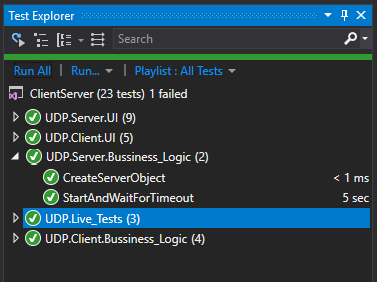
\includegraphics[width=4cm]{testexplore}
	\caption{Test explorer}
	\label{ref:visualstudiotest}
\end{center}
\end{wrapfigure}

Figure~\ref{ref:testingUDP} in the appendix contains the correctness table for the UDP Client and Server. Each test was run and the outcome was compare to what was expected. Out of 25 tests 100\% passed and produced the correct results. These tests are implemented into Visual Studio \footnote{https://www.visualstudio.com/} and are run every time a change is implemented into the server or client. Figure~\ref{ref:visualstudiotest} contains a screen shot of the test window after all tests have completed.

The degradation tool also required testing for the various effects. The effects all have a basic test that checks for a successful start up and a more in-depth test that checks the effects functionality against ping packets sent over the localhost. The two attacks also needed testing, these however do not include a test on their functionality as it would be very difficult and time consuming to create a test that tests the effectiveness of the attack. Figure~\ref{ref:testingScript} in the appendix contains the testing correctness table for the script tools; all tests passed.

\subsection{Testing methodology considerations}
Initially the methodology chosen to start development of the traffic simulation programs was ``Test Driven Development" \citep{beck2003test}, this was a tight methodology that increased development time and gave the added benefit of showing that new changes have not broken older functionality. This methodology was good to start off the project and allowed for a tight structure to be created where no time was wasted debugging previously working code, but as mentioned this methodology slowed development time down, this was chosen to be abandoned after 3-4 weeks to an ad-hoc approach. 
This change was due to time restraints on the project and the less-important role that the traffic simulation programs had on the project compared to the degradation simulation script. The degradation script was developed in the ad-hoc approach. Ad-hoc was chosen due to issues stated previously about the unknown aspects of the script and how it would operate and it was decided that the time invested to write up test scripts would assume too much and would risk them having the be completely rewritten. Tests therefore, were added alongside new functionality.





% Section Description
%
\section{Experiential design}

\subsection{Protocol Degradation}
The tool was tested against the various protocols and rough results were obtained to validate the correct function of the degradation tool. 

\subsubsection{HTTP Experiment}
HTTP traffic was tested through an automated script. The degradation tool was activated for packet loss and latency and the website was downloaded using the {\it wget} command. The website chosen was the Wikipedia page for the Univeristy of Hull \footnote{\url{https://en.wikipedia.org/wiki/University_of_Hull}}. This page was chosen due to it being a good example of a simple web page.

Appendix~\ref{ref:httpTesting} contains the results for the HTTP testing. Figure~\ref{ref:latencyHttp} contains the latency results. The page load time value is the average taken over a series of 5 repeat test. The results were as expected; the increase in load times is linear with the increase of latency.


\subsubsection{FTP Experiment}
FTP traffic was tested with two hosts connected to the Raspberry Pi router; one host the client and the other the server. Transfer speed of a 5MB file were tracked and recorded.

Appendix~\ref{ref:ftpTesting} contains the results for the experiment. As expected as the degradation becomes more violent the transfer time increases. As latency increased, transfer speed of the file decreased in a linear fashion.

\subsubsection{UDP Experiment}
UDP was tested using the custom server client created for visualising the packet loss, therefore, only packet loss was tested for UDP. In a similar way to FTP a server and client both connected to the router running the tool. The state of the user interface was recorded as significant packet loss values.

Appendix~\ref{ref:udpTesting} contains the progression of the interface as the packet loss value becomes more extreme. The clear representation of arrived and lost packets makes it immediately apparent of the effect of packet loss on a UDP connection. UDP does not resend when packets are lost, so in situations with abnormally large packet loss values an application relying on UDP can be completely incapacitated.

\subsection{Latency Accuracy}
In the initial stages of the project there were experiments that tested the effects of the degradation on the network. The tests were performed on the loopback (Internal network 127.0.0.1) with ICMP ping packets.

This test was designed to show the accuracy of different ways of simulating latency, the first way being a static timer that just causes the thread to sleep for a set amount of time or a dynamic timer that calculates the elapsed time since the creation of the thread and the command telling the thread to sleep, the dynamic timer takes this elapsed time off the target latency value.

Figure~\ref{ref:latencyAccuracy} visualises the results in a single graph. The relatively high percentage error in the small ranges of latency values is due to the error proportion being a much larger chunk of the overall target latency and therefore being a higher percentage error.

\begin{center}
	\begin{tikzpicture}[every axis plot/.append style={thick}]
		\begin{axis}[
			width=\linewidth,
			height=10cm,
			grid=major,
			xmin=1, xmax=100,
			ymin=0, ymax=100,
			xlabel=Latency (ms),
			ylabel=Error (\%)]
			\addplot table [x index=0, y index=1, mark=none, search path=csv_data, col sep=comma]{PingTestDynamicVsStatic.csv};		
			\addlegendentry{Static}	
			
			\addplot table [x index=0, y index=2, mark=none, search path=csv_data, col sep=comma]{PingTestDynamicVsStatic.csv};		
			\addlegendentry{Dynamic}	
		 \end{axis}
 \end{tikzpicture}
 
	\begin{figure}[h]
		\caption{Error percentage in simulating latency}
		\label{ref:latencyAccuracy}
	\end{figure}
\end{center}


Figure~\ref{ref:latencyAccuracy} shows the dynamic form of issuing latency is overall more accurate in simulation. However, it is still not perfect and there seems to be a small overall error present. This performance is however, more than suitable for the scope of this project.

\subsection{Visualising effects}
\begin{wrapfigure}{r}{5cm}
\begin{center}
	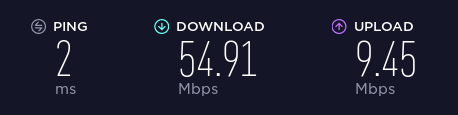
\includegraphics[scale=0.3]{SpeedNoEffect}
	\caption{The initial connection speed}
	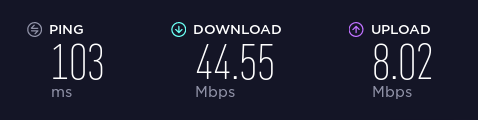
\includegraphics[scale=0.3]{Speed100ms}
	\caption{Network speed with a latency of 100ms}
\end{center}
\end{wrapfigure}

The most effective way to visualise real world connections were running tests on SpeedTest.net \footnote{\url{http://beta.speedtest.net/}}. This is very useful to quickly visualise a certain effect on the network.

As you can see from both images, the 100ms has evidently been applied effectively and the speed of the connection has dropped by around 10Mbps. This means in real world terms the time taken to download a 1GB file would take 35 seconds longer to download. This is not a considerable reduction but the latency is having an obvious effect on the network quality.


\subsection{UDP Flooding}
\begin{wrapfigure}{r}{5cm}
\begin{center}
	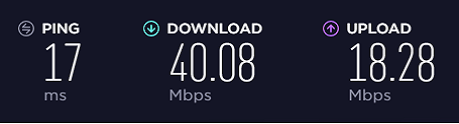
\includegraphics[scale=0.3]{before_udp}
	\caption{Initial speed without UDP flooding active}
	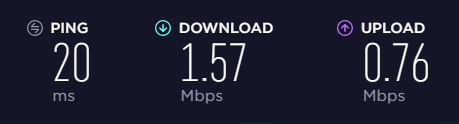
\includegraphics[scale=0.3]{after_udp}
	\caption{Speed test with UDP Flooding active}
\end{center}
\end{wrapfigure}

To test the effect of the UDP flooding required experimentation. A single target was selected on a network just containing the attacker and victim and, like previous tests, SpeedTest.Net was used to obtain bandwidth results. Each test was run with the same computers on the same network. As you can see from the two images the effect of the UDP flooding is devastating on a connections speed, taking a fast internet connection and reverting it to a crawl. If more computers running the script were active the internet connection could easily be fully blocked.